
\documentclass[a4paper,12pt]{article}
\usepackage[indonesian]{babel}
\usepackage{graphicx}
\usepackage{multirow}
\usepackage{enumitem}
\usepackage{listings}
\usepackage{wrapfig}
\usepackage[T1]{fontenc}
\usepackage{inconsolata}
\usepackage{lipsum}
\usepackage{adjustbox}


\usepackage{color}
\usepackage[table]{xcolor}
\definecolor{lightgray}{rgb}{0.95, 0.95, 0.95}
\definecolor{darkgray}{rgb}{0.4, 0.4, 0.4}
%\definecolor{purple}{rgb}{0.65, 0.12, 0.82}
\definecolor{editorGray}{rgb}{0.95, 0.95, 0.95}
\definecolor{editorOcher}{rgb}{1, 0.5, 0} % #FF7F00 -> rgb(239, 169, 0)
\definecolor{editorGreen}{rgb}{0, 0.5, 0} % #007C00 -> rgb(0, 124, 0)
\definecolor{orange}{rgb}{1,0.45,0.13}		
\definecolor{olive}{rgb}{0.17,0.59,0.20}
\definecolor{brown}{rgb}{0.69,0.31,0.31}
\definecolor{purple}{rgb}{0.38,0.18,0.81}
\definecolor{lightblue}{rgb}{0.1,0.57,0.7}
\definecolor{lightred}{rgb}{1,0.4,0.5}
\usepackage{upquote}
\usepackage{listings}
% CSS
\lstdefinelanguage{CSS}{
  keywords={color,background-image:,margin,padding,font,weight,display,position,top,left,right,bottom,list,style,border,size,white,space,min,width, transition:, transform:, transition-property, transition-duration, transition-timing-function},	
  sensitive=true,
  morecomment=[l]{//},
  morecomment=[s]{/*}{*/},
  morestring=[b]',
  morestring=[b]",
  alsoletter={:},
  alsodigit={-}
}

% JavaScript
\lstdefinelanguage{JavaScript}{
  morekeywords={typeof, new, true, false, catch, function, return, null, catch, switch, var, if, in, while, do, else, case, break},
  morecomment=[s]{/*}{*/},
  morecomment=[l]//,
  morestring=[b]",
  morestring=[b]'
}

\lstdefinelanguage{HTML5}{
  language=html,
  sensitive=true,	
  alsoletter={<>=-},	
  morecomment=[s]{<!-}{-->},
  tag=[s],
  otherkeywords={
  % General
  >,
  % Standard tags
	<!DOCTYPE,
  </html, <html, <head, <title, </title, <style, </style, <link, </head, <meta, />,
	% body
	</body, <body,
	% Divs
	</div, <div, </div>, 
	% Paragraphs
	</p, <p, </p>,
	% scripts
	</script, <script,
  % More tags...
  <canvas, /canvas>, <svg, <rect, <animateTransform, </rect>, </svg>, <video, <source, <iframe, </iframe>, </video>, <image, </image>, <header, </header, <article, </article
  },
  ndkeywords={
  % General
  =,
  % HTML attributes
  charset=, src=, id=, width=, height=, style=, type=, rel=, href=,
  % SVG attributes
  fill=, attributeName=, begin=, dur=, from=, to=, poster=, controls=, x=, y=, repeatCount=, xlink:href=,
  % properties
  margin:, padding:, background-image:, border:, top:, left:, position:, width:, height:, margin-top:, margin-bottom:, font-size:, line-height:,
	% CSS3 properties
  transform:, -moz-transform:, -webkit-transform:,
  animation:, -webkit-animation:,
  transition:,  transition-duration:, transition-property:, transition-timing-function:,
  }
}

\lstdefinestyle{htmlcssjs} {%
  % General design
%  backgroundcolor=\color{editorGray},
  basicstyle={\footnotesize\ttfamily},   
  frame=b,
  % line-numbers
  xleftmargin={0.75cm},
  numbers=left,
  stepnumber=1,
  firstnumber=1,
  numberfirstline=true,	
  % Code design
  identifierstyle=\color{black},
  keywordstyle=\color{blue}\bfseries,
  ndkeywordstyle=\color{editorGreen}\bfseries,
  stringstyle=\color{editorOcher}\ttfamily,
  commentstyle=\color{brown}\ttfamily,
  % Code
  language=HTML5,
  alsolanguage=JavaScript,
  alsodigit={.:;},	
  tabsize=2,
  showtabs=false,
  showspaces=false,
  showstringspaces=false,
  extendedchars=true,
  breaklines=true,
}
%
\lstdefinestyle{py} {%
language=python,
literate=%
*{0}{{{\color{lightred}0}}}1
{1}{{{\color{lightred}1}}}1
{2}{{{\color{lightred}2}}}1
{3}{{{\color{lightred}3}}}1
{4}{{{\color{lightred}4}}}1
{5}{{{\color{lightred}5}}}1
{6}{{{\color{lightred}6}}}1
{7}{{{\color{lightred}7}}}1
{8}{{{\color{lightred}8}}}1
{9}{{{\color{lightred}9}}}1,
basicstyle=\footnotesize\ttfamily, % Standardschrift
numbers=left,               % Ort der Zeilennummern
%numberstyle=\tiny,          % Stil der Zeilennummern
%stepnumber=2,               % Abstand zwischen den Zeilennummern
numbersep=5pt,              % Abstand der Nummern zum Text
tabsize=4,                  % Groesse von Tabs
extendedchars=true,         %
breaklines=true,            % Zeilen werden Umgebrochen
keywordstyle=\color{blue}\bfseries,
frame=b,
commentstyle=\color{brown}\itshape,
stringstyle=\color{editorOcher}\ttfamily, % Farbe der String
showspaces=false,           % Leerzeichen anzeigen ?
showtabs=false,             % Tabs anzeigen ?
xleftmargin=17pt,
framexleftmargin=17pt,
framexrightmargin=5pt,
framexbottommargin=4pt,
%backgroundcolor=\color{lightgray},
showstringspaces=false,      % Leerzeichen in Strings anzeigen ?
}%
%

\graphicspath{ {./img/} }
\begin{document}
\title{ {\Large Laporan Praktikum}\\ Algoritma dan Pemrograman Lanjut\\{\Large Pertemuan 1}}

\author{Aldzikri Dwijayanto Prathama 
	\\195410189
	\\Informatika}
\makeatletter
\begin{titlepage}
	\begin{center}
		{\huge \bfseries \@title }\\[14ex]
		
\includegraphics[scale=.8]{logo}\\[4ex]
		{\large \@author}\\[12ex]
		{\large \bfseries {SEKOLAH TINGGI MANAJEMEN INFORMATIKA DAN KOMPUTER
				AKAKOM YOGYAKARTA}}
	\end{center}


%{\large \@date} 
\end{titlepage}
\makeatother
%\maketitle
\newpage
\tableofcontents
\newpage
\section{Tujuan}
\begin{enumerate}
    \item Mengenal dan menggunakan browser
    \item Mengenal dan menggunakan editor
    \item Menulis script HTML pada editor
\end{enumerate}

\section{Dasar Teori}
\paragraph{Web\\}
Website adalah kumpulan halaman web yang dapat diakses melalui browser dan
memerlukan jaringan internet, contohnya https://www.akakom.ac.id . Cara mengakses
web terbagi atas dua bagian, yaitu sisi client serta sisi server. Script yang digunakan
untuk membuat tampilan web adalah HTML(Hypertext Markup Language).

\paragraph{HTML\\}
HTML pada dasarnya hanya file teks dengan kode yang memberi tahu browser cara
menampilkan informasi, misalnya memberi tahu browser bahwa teks tertentu harus
ditampilkan sebagai header dengan huruf tebal, atau teks diberi warna merah. Untuk
memberi tahu browser file teks berisi HTML, digunakan ekstensi file .html. Karena
dokumen HTML tidak lain adalah file teks maka dapat menggunakan editor teks apa
saja untuk membuatnya, misalnya Notepad, Microsoft Word. Struktur HTML terbagi
atas bagian

\paragraph{Browser\\}
Browser adalah program yang digunakan untuk menampilkan website. Beberapa
browser yang populer adalah Google Chrome, Firefox, Internet Explorer, Opera, dan
Safari. Melalui browser kita dapat melihat kode HTML dari sebuah web

\paragraph{Editor\\}
Digunakan untuk menuliskan kode script HTML. Editor terdiri dari duajenis, yaitu:\\
\begin{enumerate}[label=\alph*.]
    \item Text Editor : editor yang berbasis pada text saja seperti notepad. File
disimpan dengan ekstensi .html . Tampilan web bisa dilihat dari editor ,
harus dengan menggunakan browser. 
    \item Graphic User Interface : editor memiliki komponen – komponen yang dapat
di drag and drop untuk membuat sebuah halaman web. Dikenal juga
dengan istilah editor WYSIWUG . Keunggulan editor jenis ini adalah kita
sudah mendapat langsung melihat tampilan web dan kode html otomatis di
generate oleh sistem.
\end{enumerate}

\paragraph{Struktur Dokumen Html\\}
Struktur Dokumen HTML
Kode program HTML menggunakan simbol < > biasa disebut “tag” . Pengetikan kode
html bersifat insensitive case tidak membedakan huruf besar dengan huruf kecil.
Struktur penulisan html adalah sebagai berikut:
\begin{lstlisting}[frame=single,language=HTML5]
 <!DOCTYPE html>
 <html>
 <head>
 </head>
 <body>
 </body>
 </html>
\end{lstlisting}

\section{Pembahasan}
\begin{enumerate}
    \item 
        \begin{minipage}[t]{\linewidth}
              \raggedright
              \adjustbox{valign=t}{%
                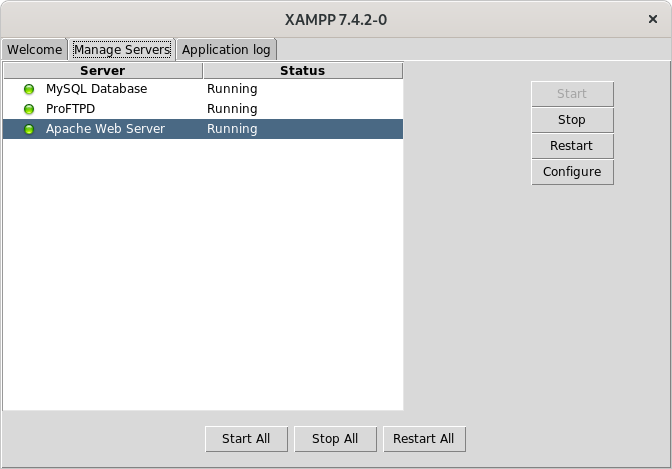
\includegraphics[width=.8\linewidth]{1.png}%
              }

              \medskip
              Nyalakan layanan apache web server. Caranya buka tab Manage Server, pilih Apache, lalu klik start.
        \end{minipage}

    \item 
        \begin{minipage}[t]{\linewidth}
              \raggedright
              \adjustbox{valign=t}{%
                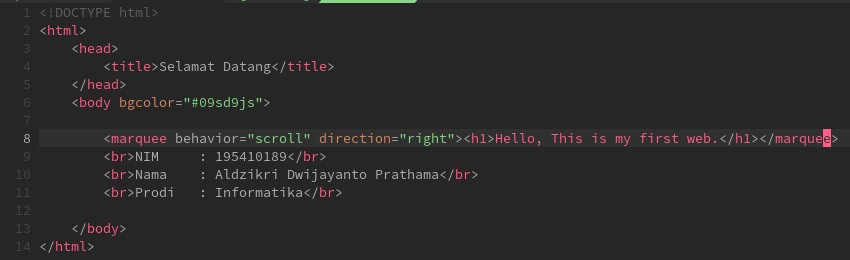
\includegraphics[width=1\linewidth]{2.png}%
              }

              \medskip
              Tulis HTML dengan menggunakan text editor. Pada html tersebut terdapat beberapa tag, diantaranya:\\
              \begin{enumerate}
                  \item <!DOCTYPE html> : menginstruksikan kepada browser tentang versi html apa halaman ditulis.
                  \item <head> : Wadah untuk semua element head.
                  \item <title> : mendefinisikan judul halaman.
                  \item <body> : elemen yang terdiri dari isi documen HTML, seperti teks, gambar, table, dll.
                  \item <marquee> : tag HTML non-standar yang digunakan untuk mebuat scrolling text.
                  \item <br> : break line
              \end{enumerate}
        \end{minipage}

    \item 
        \begin{minipage}[t]{\linewidth}
              \raggedright
              \adjustbox{valign=t}{%
                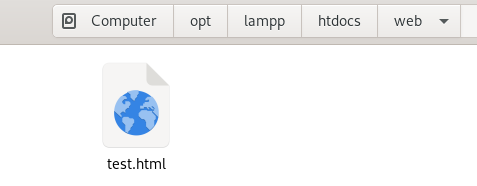
\includegraphics[width=.8\linewidth]{3.png}%
              }

              \medskip
              Simpan file html di htdocs
        \end{minipage}

    \item 
        \begin{minipage}[t]{\linewidth}
              \raggedright
              \adjustbox{valign=t}{%
                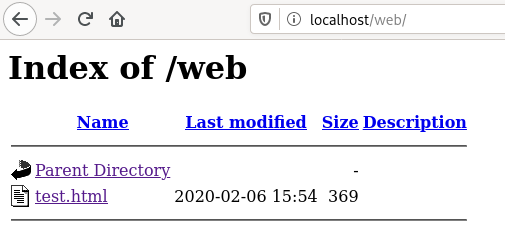
\includegraphics[width=1\linewidth]{4.png}%
              }

              \medskip
              Buka browser dan buka url localhost.
        \end{minipage}

    \item 
        \begin{minipage}[t]{\linewidth}
              \raggedright
              \adjustbox{valign=t}{%
                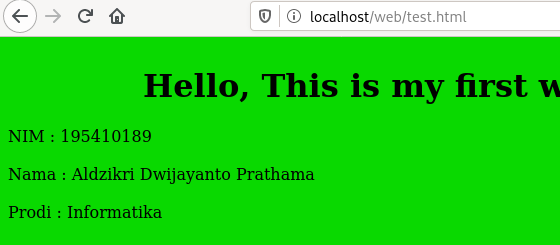
\includegraphics[width=1\linewidth]{5.png}%
              }

              \medskip
              Buka file html di browser.
        \end{minipage}
\end{enumerate}

\section{Tugas}
Carilah 2 tag , selain  <title> yang bisa diletakkan di dalam tag <head>. Sebutkan tag-nya dan berikan penjelasan\\

\paragraph{Jawab\\}
\begin{enumerate}
    \item <style> : digunakan untuk mendefinisikan informasi style untuk dokumen html.
    \item <base> : digunakan untuk menentukan base URL/target untuk semua URL dalam dokumen.
\end{enumerate}

\section{Kesimpulan}
Setelah praktikum ini mahasiswa mampu Mengenal dan menggunakan browser, dan editor. Serta menulis script HTML pada editor
\end{document}
